%=======================================
%TODO Frame 1
\begin{frame}[b]

\deuxcolonnesbottom{
\begin{minipage}[c][0.95\textheight][c]{\linewidth}
\begin{center}
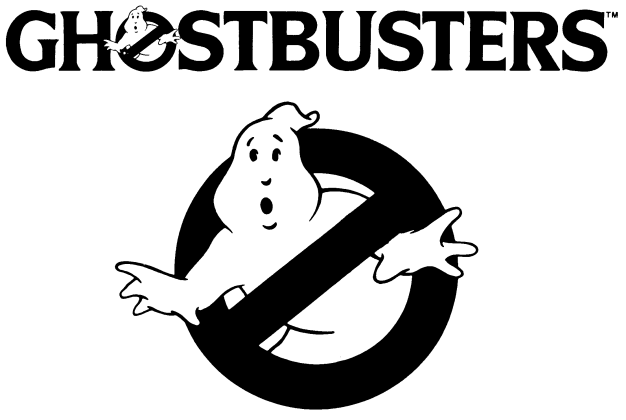
\includegraphics[width=1.0\textwidth]{ghostbusters-full.png}
\end{center}

\vspace{0.7cm}

\mysection{Introduction}

\myindent \href{https://en.wikipedia.org/wiki/Ghostbusters_(role-playing_game)}{Ghostbusters} est un jeu de rôles humoristique américain, conçu par \href{https://en.wikipedia.org/wiki/Sandy_Petersen}{Sandy Petersen}, \href{https://en.wikipedia.org/wiki/Lynn_Willis}{Lynn Willis} (les créateurs du jeu de rôles \href{https://en.wikipedia.org/wiki/Call_of_Cthulhu_(role-playing_game)}{Call of Cthulhu}), et \href{https://en.wikipedia.org/wiki/Greg_Stafford}{Greg Stafford} (le créateur de \href{https://en.wikipedia.org/wiki/RuneQuest}{Runequest} et de \href{https://en.wikipedia.org/wiki/Pendragon_(role-playing_game)}{Pendragon}), et publié en 1986 par \href{https://en.wikipedia.org/wiki/West_End_Games}{West End Games}.

\myindent Le système de jeu est très compact et très simple et vise des aventures amusantes dans l'univers des films. Il servira de fondation au \href{https://en.wikipedia.org/wiki/D6_System}{Système D6} dont \href{https://en.wikipedia.org/wiki/Star_Wars:_The_Roleplaying_Game}{Star Wars} est l'exemple le plus connu, et inspirera des dizaines de mini-jeux de rôles comme \href{https://rouboudou.itch.io/risus}{Risus}.

\myindent Ce document reprend les règles originales de 1986.

\vspace{0.2cm}

\begin{tabular}{p{3cm}p{5cm}}
Concepteur               & \copyright\ S. Petersen, L. Willis, G. Stafford \\
Version        &  Version originale 1986 \\
Traduction et adaptation & \textcopyleft\ O. Rey 2022 \\
Version                  & \myversion \\
Référence         & \myreference \\ 
\end{tabular}

\vspace{0.4cm}

%=================================================SECTION
\mysection{Création du personnage}

\mysubsection{Traits}

\myindent Les Ghostbusters possèdent quatre \textbf{Traits} :
\begin{myitemize}
\item \textbf{Cervelle} (Brains),
\item \textbf{Muscles} (Muscles),
\item \textbf{Mouvement} (Moves),
\item \textbf{Coolitude} (Cool).
\end{myitemize}

\myindent On assigne à chaque Trait une valeur numérique. Plus cette valeur est haute, meilleure est la performance du PJ qui l'utilise. Chaque joueur possède 12 points à répartir sur les 4 traits, sachant que la valeur d'un trait ne peut être ni inférieure à 1, ni supérieure à 5.

\myindent \textit{Note} : certains Ghostbusters ont plus de 5 points dans certains Traits, mais c'est le fruit de l'expérience (voir plus loin).

\myindent Lors d'une action dont l'issue n'est pas connue d'avance, le Ghostmaster assignera un \textbf{Facteur de Difficulté} (FD) à l'action. Le joueur devra lancer un nombre de \textbf{dés à 6 faces} correspondant au Trait associé, et son score devra être supérieur ou égal au FD pour que l'action réussisse.

\myindent Un de ces dés doit être un \textbf{Dé Fantôme} (DF), un dé à 6 faces de couleur différente ayant un fantôme à la place du 6 (ou géré comme tel). La valeur du fantôme est 0 (voir plus bas).

\mysubsection{Talents}

\myindent Les Ghostbusters ont un \textbf{Talent} par Trait. Quand le PJ tente une action pour laquelle il possède un Talent, le joueur lancera \textbf{3D de plus} que son Trait.

\myindent Chaque joueur doit choisir un Talent par Trait dans les listes ci-dessous. Il est possible de choisir un Talent non listé si le MJ l'accepte (dans la plupart des scénarios de Ghosbusters RPG, les PNJ ont des Talents ne figurant pas dans ces listes).
\end{minipage}
}{
\begin{minipage}[c][0.95\textheight][c]{\linewidth}
\begin{center}
\begin{tabular}{ccc}
&\textbf{Talents : Cervelle}&\\
Anthropologie & Déduction & Occultisme \\ 
Archéologie & Deviner & Parapsychologie \\
Astronomie & Électronique &  Physique \\ 
Bibliothèque scientifique & Faits sportifs & Psychanalyse \\ 
Biologie & Géologie & Réparation électrique \\
Botanique & Histoire & Réparation mécanique \\
Bureaucratie & Journalisme & Romans à l'eau de rose \\
Chimie & Linguistique & Zoologie \\
Coiffure à la mode & Mathématiques & \\
Comptabilité & Médecine & \\
\end{tabular}
\end{center}

\begin{center}
\begin{tabular}{cc>{\centering\arraybackslash}p{2.5cm}}
& \textbf{Talents : Muscles} &  \\
Bagarre & Escalader & Lutte \\
Casser des choses & Éventrer & Nager \\
Renverser à coups de pieds & Gloutonnerie & Sauter \\
Courir & Intimider & Soulever \\
\end{tabular}
\end{center}

\begin{center}
\begin{tabular}{ccc}
& \textbf{Talents : Mouvement} & \\
Attirer l'attention & Faire de la musique & Se déguiser \\
Attraper & Fouiner & Se pavaner \\
Breakdance & Furtivité & Séduire \\
Conduire (un véhicule) & Jeter & Tirer (avec une arme) \\
Écouter & Pickpocket & Tours de passe-passe \\
Équilibre & Ragots & Voir \\
Esquiver & Se cacher &  \\
\end{tabular}
\end{center}

\begin{center}
\begin{tabular}{>{\centering\arraybackslash}p{2.5cm}cc}
& \textbf{Talents : Coolitude} & \\
Bluffer & Élever des enfants & Jouer à la Bourse \\
Charmer & Emprunter & Marchander \\
Confusionner & Intimider & Orateur \\
Convaincre & Jouer au Poker & Raconter des bobards \\
\end{tabular}
\end{center}

\mysubsection{Bons Points}

\myindent Tous les Ghostbusters commencent le jeu avec 20 \textbf{Bons Points} (BP). Des BP seront gagnés quand ils auront fini les missions ou auront achevé leurs objectifs.

\myindent Quand les Ghostbusters vont mal, ils perdent des BP et prennent des amendes pour stationnement interdit, des appels injurieux de leurs créditeurs ou de longs séjours à l'hôpital.

\myindent Les Bons Points sont plus qu'une mesure de l'état de santé des Ghostbusters, ce sont des moyens pour eux d'influer sur l'histoire, de les voir tenter d'incroyables prouesses ou de les sortir de terribles ennuis.

\begin{center}
\begin{tabular}{cc}
\textbf{Action} & \textbf{Coût en BP}\\
Augmenter ses chances de succès\textsuperscript{1} & 1 BP = +1D au jet \\
Réduire le temps de séjour à l'hôpital & 1 BP = $-1$ semaine \\
Compenser une action très stupide & Un certain nombre de BP \\
Éviter de mourir & Un certain nombre de BP \\
\end{tabular}
\end{center}

{\small \textit{\textsuperscript{1} La décision de dépenser des Bons Points doit être faite avant le jet et ne peut pas modifier un jet déjà réalisé.}}

\mysubsection{Liens entre Bons Points et Traits}

\myindent Les Traits sont liés avec les BP de la manière suivante (avec accord du Ghostmaster) :

\begin{center}
\begin{tabular}{ccc}
\textbf{Contexte} & \textbf{Action} & \textbf{Impact en BP}\\
Expérience & Faire +1 sur un Trait & $-30$ BP \\
Moment critique\textsuperscript{2} & Faire $-1$ sur un Trait & +20 BP \\
\end{tabular}
\end{center}

{\small \textit{\textsuperscript{2} Par exemple, au lieu de mourir, un Ghostbuster n'ayant plus de BP peut en retrouver en perdant définitivement 1 point sur un de ses Traits.}}

\myindent Quand les BP sont utilisés par les joueurs pour sortir le Ghostbuster d'une mauvaise situation, ces derniers doivent décrire la situation. Si la description est amusante, le Ghostmaster pourra gratifier le Ghostbuster d'un bonus de +1 ou +2 BP.

\mysubsection{Expérience}

\myindent Le gain de BP après une mission est évalué comme suit :

\begin{center}\begin{tabular}{>{\centering\arraybackslash}p{3cm}>{\centering\arraybackslash}p{5cm}}
\textbf{Situation} & \textbf{Gain en BP}\\
Mission échouée ou fantôme non capturé & La moitié des BP perdus pendant la mission \\
Mission réussie & La totalité des BP récupérés, voire un léger bonus \\
Mission accomplie avec panache et fun & Tous les BP sont récupérés + la moitié des BP perdus pendant la mission \\
\end{tabular}
\end{center}
\end{minipage}
}
\end{frame}

%=======================================
%=======================================
%TODO Frame 2
\begin{frame}[b]

\deuxcolonnesbottom{%col1
\begin{minipage}[c][0.95\textheight][c]{\linewidth}
\mysubsection{Objectif Personnel}

\myindent Le Ghostbuster poursuit un \textbf{Objectif Personnel}. L'atteindre lui accordera de nouveaux BP. La liste est donnée ci-dessous, sachant que le Ghostmaster peut valider un objectif n'étant pas dans la liste.

\myindent \textbf{Sexe} -- Le Ghostbuster est habitué à des relations sans lendemain. Si le Ghostbuster réussit à avoir un rendez-vous amoureux qui se passe bien durant une aventure : +1DF en BP. Si le Fantôme est tiré, le Ghostbuster fait une grosse bêtise pendant le rendez-vous et ne gagne pas de BP (mais en gagnera un de plus au prochain jet réussi).

\myindent \textbf{Richesse} -- Le Ghostbuster est attiré par les richesses. Le Ghostmaster peut récompenser le Ghostbuster qui gagne de l'argent ou qui gagne à la bourse. Bien entendu, en cas de retournement de fortune, le Ghostmaster pourra pénaliser le Ghostbuster de quelques BP.

\myindent \textbf{Célébrité} -- Le rêve du Ghostbuster est d'être un héros des médias, d'être reçu par le Président, etc. Ce dernier gagne 1DF de BP quand il passe dans les médias locaux et 2D quand il passe dans les médias nationaux (dont le DF). S'il fait la une d'un journal international comme \textit{Time}, il peut gagner jusqu'à 6DF ou plus (dont le DF) ! En cas de tirage du Fantôme, le Ghostbuster est ridiculisé et il ne gagne aucun BP.

\myindent \textbf{Science sans conscience} -- Le Ghostbuster pense que la science passe avant tout, sans préoccupation pour l'impact sur les gens alentour. Une découverte en fantômologie fera gagner 1DF en BP au Ghostbuster, et une découverte majeure pourra lui faire gagner plus (à la discrétion du Ghostmaster). Si le Fantôme est tiré, aucun gain de BP n'est réalisé mais un point de plus sera gagné au prochain jet réussi.

\myindent \textbf{Servir l'Humanité} -- Le Ghostbuster est intéressé par faire le bien, sauver le monde, etc. A la fin de chaque aventure, le Ghostbuster reçoit 1DF de BP par ennemi de l'humanité vaincu. Si l'ennemi était particulièrement coriace, il est possible que Ghostmaster accorde plus. Une victoire sur une agence gouvernementale peut aussi apporter un bonus de BP.

\mysubsection{Personnalité et photo}

\myindent Le joueur doit déterminer la personnalité de son Ghostbuster, potentiellement ajouter une photo, remplir sa ficher de personnage (voir autre PDF) et le tour est joué.

%=================================================SECTION
\mysection{Les règles}

\mysubsection{Faire des choses}

\myindent Les tâches pour lesquelles l'issue n'est pas évidente se voient attribuer un \textbf{Facteur de Difficulté} (FD) par le Ghostmaster suivant la table ci-dessous :

\begin{center}
\begin{tabular}{>{\centering\arraybackslash}p{3cm}>{\centering\arraybackslash}p{3cm}}
\textbf{Type de tâche} & \textbf{FD}\\
Tâche facile & 5 ou plus \\
Tâche normale & 10 ou plus \\
Tâche difficile & 20 ou plus \\
Tâche impossible & 30 ou plus \\
\end{tabular}
\end{center}

\mysubsection{Influence du Dé Fantôme (DF)}

\begin{center}
\begin{tabular}{p{3.5cm}p{4.5cm}}
\textbf{Type de tirage} & \textbf{Conséquence}\\
Pas de Fantôme & Ajouter les chiffres et comparer au FD \\
Fantôme et somme des autres dés supérieure ou égale au FD & Succès accompagné d'un petit quelque chose d'ennuyeux \\
Fantôme et somme des autres dés inférieure au FD & Échec et quelque chose de mauvais arrive \\
\end{tabular}
\end{center}

\myindent Le Dé Fantôme marche de manière inversée pour les revenants : il garde sa valeur 0 mais provoque quelque chose de bon pour eux.

\mysubsection{Duels}

\myindent Le Duel peut se dérouler sur tous les niveaux : mots, poings, cervelle, habileté, argent, ou quoique ce soit d'autre. 

\end{minipage}
}
{
\begin{minipage}[c][0.95\textheight][c]{\linewidth}
\myindent Le Ghostmaster décide quel Trait ou Talent est applicable pour chacun des protagonistes. Chaque duelliste lance ses dés (incluant le DF) et le plus haut score gagne. Si les protagonistes sont ex-æquo, selon les cas, le Ghostmaster laissera en l'état ou fera rejouer. Il traitera aussi les cas de fantôme tirés sur le DF.

\mysubsection{Mouvement}

\myindent Plus le score de Mouvement est élevé et plus le Ghostbuster est rapide. La gestion des mouvements est laissée à l'appréciation du Ghostmaster.

\mysubsection{Séquence de jeu}

\myindent La séquence de jeu est la suivante :

\begin{center}
\begin{tabular}{c p{7.5cm}}
\textbf{\#} & \textbf{Explication}\\
1 & Le Ghostmaster annonce ce que vont faire les PNJ (personnages ou fantômes) \\
2 & Le Ghostmaster demande à chaque joueur en commençant par sa droite ce que les Ghostbusters comptent faire \\
3 & Le Ghostmaster décide qui va faire quoi à qui et dans quel ordre et quels dés doivent être lancés \\
\end{tabular}
\end{center}

\myindent Durant les séquences d'action, chaque Ghostbuster peut faire un déplacement et une action.

\myindent Il y a deux types de combats : les \textbf{mêlées} et les \textbf{combats à distance}.

\mysubsection{Mêlée}

\myhl{Muscles}{Bagarre}

\myindent Si un adversaire ou un Ghostbuster utilise un gourdin, alors ce dernier aura un avantage plus ou moins important (voir table ci-dessous).

\begin{center}
\begin{tabular}{c p{6.5cm}}
\textbf{Bonus} & \textbf{Armes}\\
+1D & Poing américain, matraque, ongles longs \\
+2D & Cran d'arrêt, fouet, poêle à frire \\
+3D & Gourdin, chaise, épée \\
+4D & Hache de bataille, tronçonneuse, perceuse électrique \\
\end{tabular}
\end{center}

\mysubsection{Combat à distance}

\myhl{Mouvement}{Tirer}

\myindent Le FD varie suivant la portée du tir.

\begin{center}
\begin{tabular}{l p{5.5cm} c}
\textbf{Distance} & \textbf{En mètres} & \textbf{FD} \\
Bout-portant & Moins de 3m & 5 \\
Normale & Entre les deux & 10 \\ 
Longue & 15m ou plus pour un pistolet, fusil à canon scié, or canon à proton (\textit{proton-pack}), 150m pour un fusil &  20 \\
\end{tabular} \\
\end{center}

\mysubsection{Mort, dommages, hôpital et maladie}

\myindent Les Ghostbusters ne meurent généralement jamais (les fantômes non plus d'ailleurs, ils le sont déjà). Par contre, ils sont blessés, le matériel est endommagé ou détruit et les fantômes sont engloutis par le piège à fantômes.

\myindent Pour autant, en cas d'abus d'un joueur, le Ghostmaster pourra faire mourir le PJ qui, après des funérailles touchantes, pourra hanter ses anciens amis.

\begin{center}
\begin{tabular}{>{\raggedright\arraybackslash}p{2cm} p{6cm}}
\textbf{Dommages} & \textbf{Perte en BP}\\
Touché par une hache de guerre & De 1 à 10 (membre sectionné mais recollable en hôpital) suivant la gravité \\
Chute & 1 BP par 5 mètres avec un maximum de 5 BP (quelque soit la hauteur) \\
Feu, radioactivité & 1 BP par brûlure avec un maximum de 20. La radioactivité a un effet retard (le MJ peut la gérer sans que les joueurs ne soient au courant jusqu'à apparition des symptômes) \\
Noyade, asphyxie & 1 BP par minute sans respirer jusqu'à un maximum de 10 \\
Poison & 1 BP si le poison fait juste mal ventre, jusqu'à 10 ou 15 BP pour les poisons les plus violents \\
\end{tabular}
\end{center}

\end{minipage}
}
\end{frame}

%=======================================
%=======================================
%TODO Frame 3
\begin{frame}[b]

\deuxcolonnesbottom{%col1
\begin{minipage}[c][0.95\textheight][c]{\linewidth}
\mysubsection{Équipement}

\myindent Les Ghostbusters ne peuvent porter que 3 objets sans pénalité (au maximum un nombre d'équipements égal à leurs \textit{Muscles} mais sans possibilité d'action autre que bouger et grommeler).


\begin{wrapfigure}{l}{5cm}
%\centering
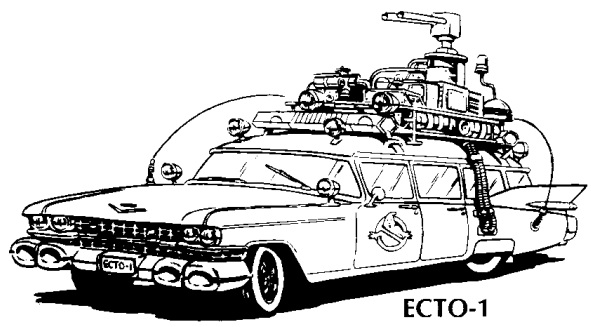
\includegraphics[width=0.5\textwidth]{./images/ECTO-1.png}
\end{wrapfigure}

\myindent Les Ghostbusters possèdent une voiture toute équipée, ECTO-1, qui normalement propose 3 places confortables, pour monter à 6 dans les moments critiques.

\myindent Par contre, cet engin est tout sauf discret.

\begin{center}
\begin{tabular}{>{\raggedright\arraybackslash}p{1.8cm} p{6cm}}
\textbf{Équipement} & \textbf{Caractéristiques}\\
Kit d'escalade & +3D en \myhl{Muscles}{Escalade} \newline
Fonctionne sur les montagnes, les buildings, les ascenseurs. Comporte des pitons, des marteaux, des cordes, des harnais et même un short bavarois.\\
Analyseur d'auras (\textit{Aura Video-Analyzer})& Un écran et un casque. Révèle les sentiments et les mensonges de celui qui porte le casque. Révèle l'archétype du personnage ; s'il est possédé, l'archétype de ce qui le contrôle.\\
Kit de plage & Un ballon et un filet de volleyball ; des lunettes de soleil, de la crême solaire, un parasol, des grandes serviettes, un frisbee, une radio. \\
Un mégaphone & Pour se faire entendre des gens et des fantômes. \\
Un téléphone cellulaire de voiture & Malgré le prix de l'abonnement, cet équipement est le signe d'un certain niveau social (en 1986). \\
Compteur \newline Geiger & Pour les endroits radioactifs ou les accélérateurs de particules pirates. \\
Piège à fantôme (\textit{Ghost Trap})& Une petite boîte reliée à une pédale par un fil d'environ 3 mètres. Quand on appuie sur la pédale, le piège s'ouvre et produit un cône de force psycho-cinétique attirant le fantôme à l'intérieur. Mais comme le fantôme peut bouger et s'éloigner, il est bon de le retenir avec un canon à protons. Quand on lève le pied de la pédale, le piège se referme. \\
\end{tabular}
\end{center}

\begin{center}
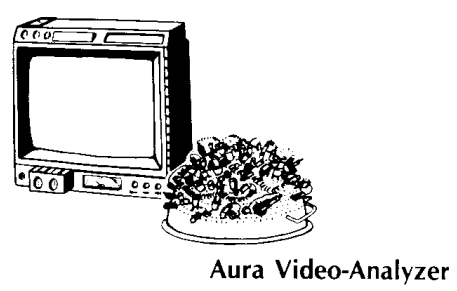
\includegraphics[width=0.4\textwidth]{./images/aura-analyseur.png} \hspace{0.5cm}  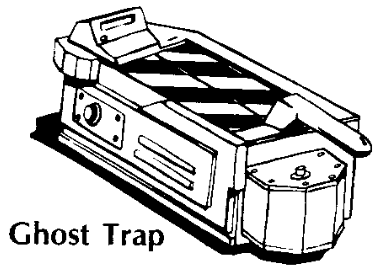
\includegraphics[width=0.28\textwidth]{./images/ghost-trap.png}\textsl{}
\end{center}

\begin{center}
\begin{tabular}{>{\raggedright\arraybackslash}p{1.8cm} p{6cm}}
\textbf{Équipement} & \textbf{Caractéristiques}\\
Caméra infrarouge & Ces caméra peuvent filmer les fantômes dans l'obscurité, même lorsque ceux-ci sont invisibles. Elle peut être pilotée à distance (FD = 10) et réglée pour prendre des photos à intervalles réguliers (FD = 10) \myhl{Cervelle}{Photographie}. \\
Canon à proton (\textit{Proton Pack}) & Petits accélérateurs de particules non autorisés, les canons à protons sont l'arme de base du Ghostbuster. Le canon à proton fait énormément de dégâts (sur les murs, les boiseries, l'ameublement) et parfois il permet de maîtriser les fantômes. En mode "attaque", et à la suite d'un jet réussi, le canon à protons  permet de faire diminuer l'Ectoprésence (EP) du fantôme de 1. En mode "confinement", deux Ghostbusters au moins doivent coopérer pour emprisonner un fantôme ayant une EP de 0 dans les rayons du canon (si l'EP du fantôme n'est pas 0, il s'enfuit). Le fantôme peut alors être placé dans un piège. \newline Croiser des rayons de canons en mode attaque génère une explosion énorme (conditions : le faire volontairement ; ou chaque Ghostbuster tire sur la même cible dans le même round et le jet est un Fantôme). \newline Voir page suivante : \textit{utilisation du canon à protons}. \\
\end{tabular}
\end{center}

\end{minipage}
}{%col2
\begin{minipage}[c][0.95\textheight][c]{\linewidth}
\begin{center}
\begin{tabular}{>{\raggedright\arraybackslash}p{1.8cm} p{6cm}}
\textbf{Équipement} & \textbf{Caractéristiques}\\
Enclos grillagé à fantômes (\textit{Protection Grid}) & Peut contenir un très grand nombre de fantômes. Il se peut qu'après de très nombreuses aventures, il soit plein et menace de s'effondrer, mais seul le Ghostmaster sait ce qui peut se passer. \\
Appareil de Mesure d'Énergie Psychokinétique (\textit{PKE-meter}) & Outil pour détecter les fantômes en mesurant les valences psychokinétiques. Quand un fantôme est dans le coin, les lumières de l'outil clignotent et les bras se lèvent (en fonction de la puissance du fantôme). \\
Parachute & Fonctionne si un DF n'est pas tiré. \\
Des lunettes d'Ectovision & Permettent de voir dans le noir. Éliminent la vision latérale. Font paraître un peu idiot.\\
Équipement de plongée sous-marine & Combinaison, palmes, bouteille d'oxygène (30 min), masque, sont utiles pour les investigations dans les égouts, la mer ou autre situation de fantômes aquatiques. Jet de \myhl{Muscles}{Nager} pour utilisation. \\
Livres secrets de sciences occultes & Chaque bon occultiste a au moins un livre occulte. Quelques exemples : \textit{Guide des sociétés secrètes et des sectes} par Roylance ; \textit{Guide des revenants} par Tobin ; \textit{Le catalogue Spates des horreurs sans nom} par Spates ; \textit{Le grand livre des sciences occultes} par Fredde ; etc. Les livres peuvent contenir des indices ou même être la source d'aventures. \\
Caméra vidéo & Peut servir à enregistrer une activité de fantômes (pour ceux qui se voient à la caméra) ou à tourner une publicité. \\
Talkies-Walkies & Absolument nécessaire quand le groupe doit se séparer. Portée : quelques centaines de mètres. Capte aussi les conversations des camionneurs, beaucoup de grésillements et ne fonctionne plus en présence de forces psychokinétiques. \\
\end{tabular}
\end{center}

\begin{center}
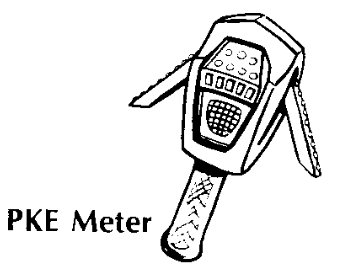
\includegraphics[width=0.3\textwidth]{./images/pke.png} \hspace{0.5cm}  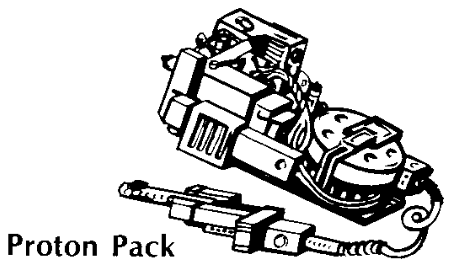
\includegraphics[width=0.4\textwidth]{./images/proton.png}\textsl{}
\end{center}

\myindent Des nouveaux équipements, plus ou moins fiables, peuvent être donnés aux Ghostbusters pour une mission spécifique par Ghostbusters Intermational (GBI) Research Labs ou la franchise locale.

\myindent Vous pouvez aussi inventer un appareil. Dans ce cas, proposez trois ou quatre concepts d'appareils au Ghostmaster, décrivez le principe pseudo-scientifique sur lequel ils s'appuient, le projet de recherche et l'argent que vous êtes prêt à investir dedans. Le Ghostmaster vous dira si l'un d'entre eux fonctionne, comment et si des effets indésirables (comme des explosions) ont été à déplorer dans le cours du projet.

\mysection{Notions de fantômologie}

\mysubsection{Ectoprésence}

\myindent Au cœur de l'aventure se trouve un fantôme, un démon, un alien, le Monstre du Loch Ness ou une autre créature. La plupart des fantômes ont une \textbf{Ectoprésence} (EP), qui quantifie leur indice de pénétration dans notre monde. Plus l'EP d'un fantôme est élevée, plus il est difficile de le soumettre.

\begin{center}
\begin{tabular}{>{\raggedright\arraybackslash}p{1.8cm} p{6cm}}
\textbf{Ectoprésence} & \textbf{Solution}\\
1 à 5 & Une multiple application du canon à proton suffit \\
6 à 10 & Opposant sérieux \\
Plus & Très compliqué \\
Zuul & Probablement une EP de plus de 100 ! Nécessaire d'avoir uns stratégie pour le combattre \\
\end{tabular}
\end{center}

\myindent Un fantôme, une fois touché par un canon à protons, cherchera à s'enfuir. Il régénère un point de EP par heure après avoir été touché.
\end{minipage}
}
\end{frame}


%=======================================
%=======================================
%TODO Frame 4
\begin{frame}[b]
\deuxcolonnesbottom{%col1
\begin{minipage}[c][0.95\textheight][c]{\linewidth}
\mysubsection{Objectif personnel}

\myindent Tous les fantômes ont un objectif personnel qui va souvent au delà des objectifs personnels des Ghostbusters. Cet objectif est lié à l'histoire du fantôme et le comprendre pourra permettre de le vaincre ou de le libérer. Connaître le but d'un fantôme permet au Ghostmaster de donner du sens à l'aventure.

\myindent Les fantômes simples ont des objectifs simples, souvent pilotés par les 7 péchés capitaux : colère, avarice, envie, gourmandise, luxure, orgueil, paresse. Les fantômes avec un pouvoir plus important (3 ou plus)  ont souvent des buts plus élaborés.

\mysubsection{Utilisation du canon à protons}

\myhl{Mouvement}{Tirer}

Les \textbf{Dommages} (DOM) faits aux fantômes dépendent de la marge de succès du jet (perte de N EP si jet du Ghostbuster $\geq$ NxFD).

\begin{center}
\begin{tabular}{cccccccc}
\textbf{Type} & \textbf{FD} & \textbf{DOM} & \textbf{2xFD} & \textbf{DOM} & \textbf{3xFD} & \textbf{DOM}\\
Cible fixe & 5 & -1EP & 10 & -2EP & 15 & -3EP\\
Cible mouvante & 10 & -1EP & 20 & -2EP & 30 & -3EP\\
Fantôme agile & 15 & -1EP & 30 & -2EP & 45 & -3EP\\
Longue portée & 20 & -1EP & 40 & -2EP & 60 & -3EP\\
Les yeux fermés & 30 & -1EP & 60 & -2EP & 90 & -3EP\\
\end{tabular}
\end{center}

\mysubsection{Autres méthodes}

\myindent Les exorcismes et les rituels de bannissement fonctionnent aussi parfois sur les créatures. Plus la solution pour vaincre la créature est dramatique et amusante, plus elle doit être récompensée par le Ghostmaster.

\mysubsection{Pouvoir et Capacité}

\myindent Les fantômes ont tous un score de \textbf{Pouvoir} montrant leur capacité de manipulation de l'énergie psychokinétique.

\myindent Chaque fantôme a, de plus, une ou des \textbf{Capacités} (généra-lement une par point de Pouvoir).

\myindent Pour les utiliser, le Ghostmaster détermine un FD et lance le nombre de dés correspondant au Pouvoir, en incluant le DF. Si le jet rate, soyez créatif et amusant. Si le DF est tiré avec un échec, la situation doit tout de même favoriser un peu le fantôme.

\myindent La durée moyenne d'une Capacité est de 5 x POU minutes (quand applicable).

\begin{center}
\begin{tabular}{clcl}
\textbf{1D} & \textbf{Capacité I} & \textbf{1D} & \textbf{Capacité II (plus puissant)} \\
1 & Slime & 1 & Lire les pensées \\
2 & Terroriser & 2 & Créer des illusions \\
3 & Matérialiser & 3 & Invoquer des nuisibles \\
4 & Posséder & 4 & Animer \\
5 & Poltergeist & 5 & Contrôler l'esprit \\
6 & Dématérialiser un objet & 6 & Murphy \\
\end{tabular}
\end{center}

\myindent Les listes ci-dessus sont donnés à titre indicatif mais d'autres Capacités peuvent être créés par le Ghostmaster.

\begin{center}
\begin{tabular}{c p{5.9cm} >{\raggedright\arraybackslash}p{1.5cm}}
\textbf{C.} & \textbf{Caractéristiques} & \textbf{Avec DF}\\
\rotatebox[origin=rB]{90}{Slime} & Produit ectoplasmique gluant, gélatineux et dégoûtant détériorant les tapis, la nourriture et engluant les Ghostbusters. Un fantôme peut engluer une personne ou un objet par attaque, avec une nécessité d'être proche de la cible (bout-portant) avec un FD=5. \newline En cas de succès du fantôme, la Coolitude du Ghostbuster est divisée par deux (arrondie au dessus) tant que le Slime n'est pas enlevé. Son costume est fichu. & Le Ghostbuster est paralysé et doit être aidé pour se désengluer.  \\
\rotatebox[origin=rB]{90}{Matérialiser} & Le fantôme se matérialise dans un squelette dansant, une statue ou autre. Généralement, les fantômes n'ont qu'une seule matérialisation, qui permet au fantôme de causer des dommages physiques (tout en restant sensible au canon à protons). Le fantôme possède temporairement deux Traits (Muscles et Mouvement) à la valeur de son Pouvoir et ne peut pas prendre de dommages. \newline Durant les quelques secondes qui lui permettent de redevenir fantôme, il est possible de tenter quelque chose contre lui. & \\
\rotatebox[origin=rB]{90}{Animer} & Un fantôme peut animer un certain nombre d'objets : faites une jet de Pouvoir pour déterminer ce nombre. Avec ces objets, le fantômes peut attaquer les Ghostbusters à la discrétion du Ghostmaster. & Nombre d'objets = double du jet de Pouvoir.\\
\end{tabular}
\end{center}
\end{minipage}
}{
\begin{minipage}[c][0.95\textheight][c]{\linewidth}
\begin{center}
\begin{tabular}{c p{5.9cm} >{\raggedright\arraybackslash}p{1.5cm}}
\textbf{C.} & \textbf{Caractéristiques} & \textbf{Avec un DF}\\
\rotatebox[origin=rB]{90}{Terroriser} & Le fantôme est soit effrayant par nature, soit il est capable de se transformer en quelque chose d'effrayant. Le fantôme tente un Duel Pouvoir/Coolitude avec chaque personne exposée. \newline En cas d'échec, la personne est immunisée 30 minutes ; en cas de réussite, elle panique et s'enfuie (30 minutes pour revenir à ses esprits). & En cas de succès du fantôme, la personne s'évanouit. \\
\rotatebox[origin=rB]{90}{Possession} & Pour posséder une personne, un fantôme doit réussir un Duel Pouvoir/Cervelle. En cas d'échec, il ne peut retenter avant au moins 1 heure. En cas de réussite, le fantôme utilise les Muscles et Mouvement de la personne mais la Cervelle et la Coolitude sont remplacées par le Pouvoir du fantôme. \newline Le fantôme n'a aucun accès à la mémoire, la personnalité ou les connaissances du possédé.
& Echec + DF : le fantôme peut retenter une possession quand il le souhaite. \\
\rotatebox[origin=rB]{90}{Poltergeist} & Spécialisation en lévitation et télékinésie. Les fantômes vandales adorent ce Pouvoir pour jeter des objets, tout casser ou animer des choses de façon amusante. Chaque action a un FD (5 pour soulever un petit objet, variable pour lancer plusieurs objets à la fois, 50 pour faire trembler le pont de Brooklyn). Si le fantôme jette des objets sur un Ghostbuster, faire un Duel Muscles/Pouvoir pour voir si l'attaque réussit. & \\
\rotatebox[origin=rB]{90}{Dématér.} & Suivant la taille de l'objet, le dématérialiser nécessite un FD différent (5 pour un magnet, 10 à 15 pour un frigo, etc.). Seuls des objets peuvent être dématérialisés. Ils réapparaissent ensuite à des endroits incongrus. & \\
\rotatebox[origin=rB]{90}{Lire les pensées} & Pour réussir, le fantôme doit gagner un Duel Pouvoir/Cervelle. Il découvre alors tous les plans de la personne. \newline Comme la personne touchée sait que ses pensées sont lues (sauf DF), elle peut résister en faisant un Duel Coolitude/Pouvoir et en se concentrant sur autre chose (demander au joueur). & La personne ne sait pas que ses pensées sont lues ; elle ne peut pas résister.  \\
\rotatebox[origin=rB]{90}{Créer illusions} & Un fantôme possède généralement une ou deux illusions en cohérence avec son objectif personnel. Suivant la complexité de l'illusion, le FD est différent (5 pour un brouillard léger, 20 pour un ptérodactyle volant autour d'un building). \newline Il est possible de voir que c'est une illusion en gagnant un Duel Cervelle/Pouvoir contre le fantôme. & \\
\rotatebox[origin=rB]{90}{Invoq. nuisibles} & Le fantôme peut invoquer et contrôler un type de nuisibles : des hordes de cafards ou de rats, des nuages de mouches, des centaines d'araignées, des chats hurlants, des amas de serpents, des vagabons, des représentants en assurance, etc. \newline Le FD dépend de la difficulté de la tâche et du lieu. & \\
\rotatebox[origin=rB]{90}{Contrôle} & Pour que le fantôme réussisse à contrôler l'esprit d'une personne, il doit réussir un Duel Pouvoir/Coolitude. Ce n'est pas une possession, mais le fantôme peut faire faire n'importe quoi à la personne. & \\
\rotatebox[origin=rB]{90}{Murphy} & Ce pouvoir permet aux fantômes de déclencher la loi de Murphy sur les objets : un canon à proton cesse de fonctionner, des machines se mettent à dysfonctionner, etc. Le Ghostbuster décide de la difficulté à causer ces problèmes et assigne un FD. & \\
\end{tabular}
\end{center}

\mysubsection{Vraies mauvaises nouvelles : démons, horreurs surnaturelles et comptables}

\myindent Les démons et autres horreurs sont plus compliquées à combattre, aussi en raison de leur puissance et de leurs serviteurs. La plupart des démons sont bavards et prétentieux. Ils ont leur propre personnalité, leur objectif, leurs défauts, leurs manies et obsessions, et leur vocabulaire propre. Ils ne peuvent être vaincus que par une conjonction de moyens dont les appareils scientifiques loufoques, les rituels et les canons à protons.

\mysubsection{Exemples de fantômes}

\vspace{-0.5cm}

\begin{center}
\begin{tabular}{l>{\centering\arraybackslash}p{2.2cm}>{\centering\arraybackslash}p{3.8cm}}
& \textbf{Luigi Elgato} & \textbf{Tammanung} \\
Type et objectif & Metteur en scène revanchard & Chef indien voulant retrouver sa terre\\
Pouvoir & 3 & 5\\
Capacités & Slime, Poltergeist & Utilisation des armes, terroriser, danse de la pluie \\
Ectoprésence & 4 & 8\\
\end{tabular}
\end{center}
\end{minipage}
}

\end{frame}
